\section{Time Reduction}\label{sec:time_reduction}

\subsection{Training Phase}
Using the \textbf{FP8} format noticeably accelerates training while lowering GPU memory requirements, even though the hardware configuration remains unchanged. As reported in Figure~\ref{fig:training_time_reduction}, the wall-clock time per epoch decreases when moving from \textbf{BF16} to \textbf{FP8}, whereas Figure~\ref{fig:losses_comparison} shows that all precisions follow essentially the same loss curve. In practice, the FP8 run completes an epoch roughly 27\,\% faster than BF16 and more than twice as fast as FP32, yet never exceeds 60\,\% of the memory consumed by FP32.

\begin{figure}[h]
    \centering
    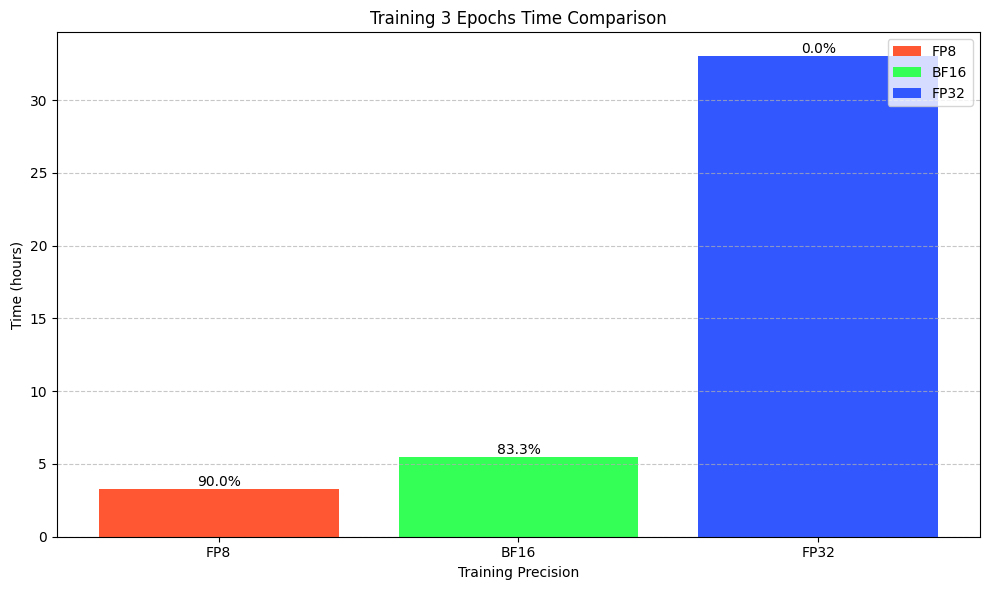
\includegraphics[width=0.75\linewidth]{figures/c4/training_time_reduction.png}
    \caption{Wall-clock training time per epoch in FP32, BF16, and FP8.}
    \label{fig:training_time_reduction}
\end{figure}

\begin{figure}[h]
    \centering
    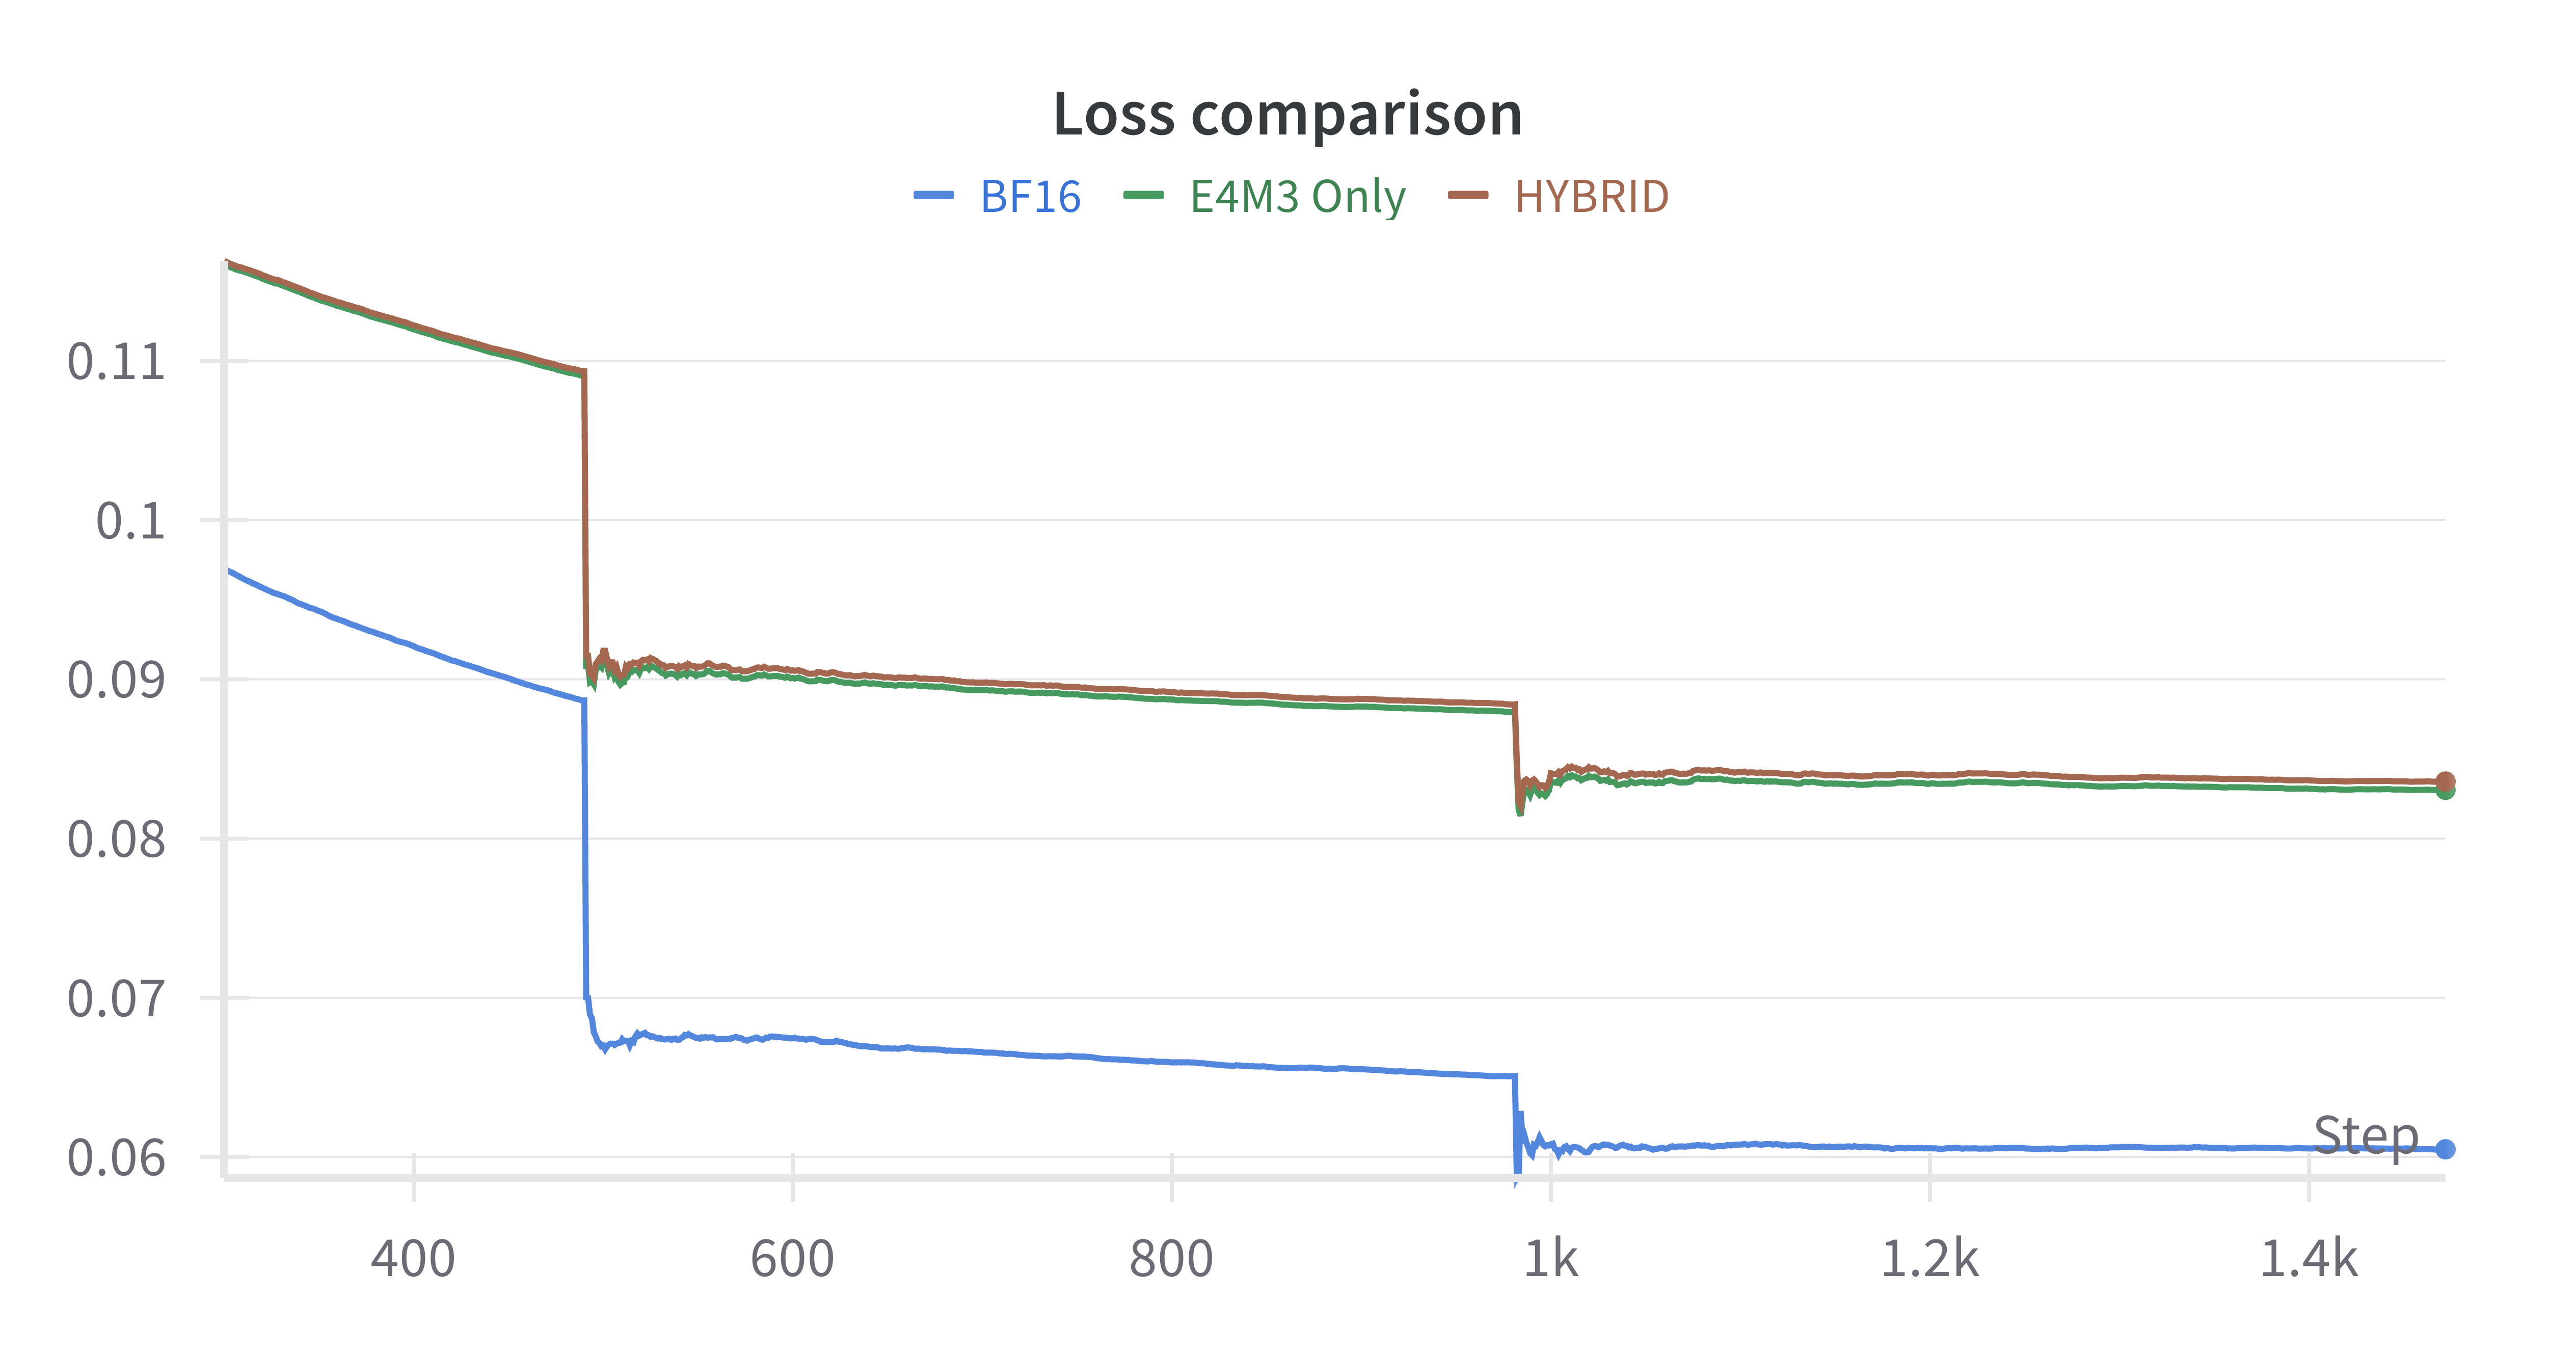
\includegraphics[width=1\linewidth]{figures/c4/losses_comparison.png}
    \caption{Validation loss versus training steps for the three precisions.}
    \label{fig:losses_comparison}
\end{figure}

\subsection{Inference Phase}
Inference benchmarks confirm the same trend. Table~\ref{tab:inference-benchmark} summarizes throughput and peak memory, while Figure~\ref{fig:inference_benchmark} provides a visual comparison. Running in FP8 sustains \textbf{102.49\,tokens/s} and requires only \textbf{1.70\,GiB}, making it about 2.5\,times faster and 3.4\,times more memory-efficient than FP32. FP16 offers intermediate performance, delivering 76.31\,tokens\,s$^{-1}$ with a 2.91\,GiB footprint. These figures demonstrate that FP8 combines the highest speed with the lowest memory cost, all without degrading accuracy.

\begin{table}[h]
    \centering
    \begin{tabular}{|c|c|c|}
        \hline
        \textbf{Precision} & \textbf{Speed (tokens/s)} & \textbf{Memory (GiB)} \\
        \hline
        FP8  & \textbf{102.49} & \textbf{1.70} \\
        FP16 & 76.31           & 2.91          \\
        FP32 & 41.27           & 5.84          \\
        \hline
    \end{tabular}
    \caption{Inference throughput and memory usage across numerical precisions.}
    \label{tab:inference-benchmark}
\end{table}

\begin{figure}[h]
    \centering
    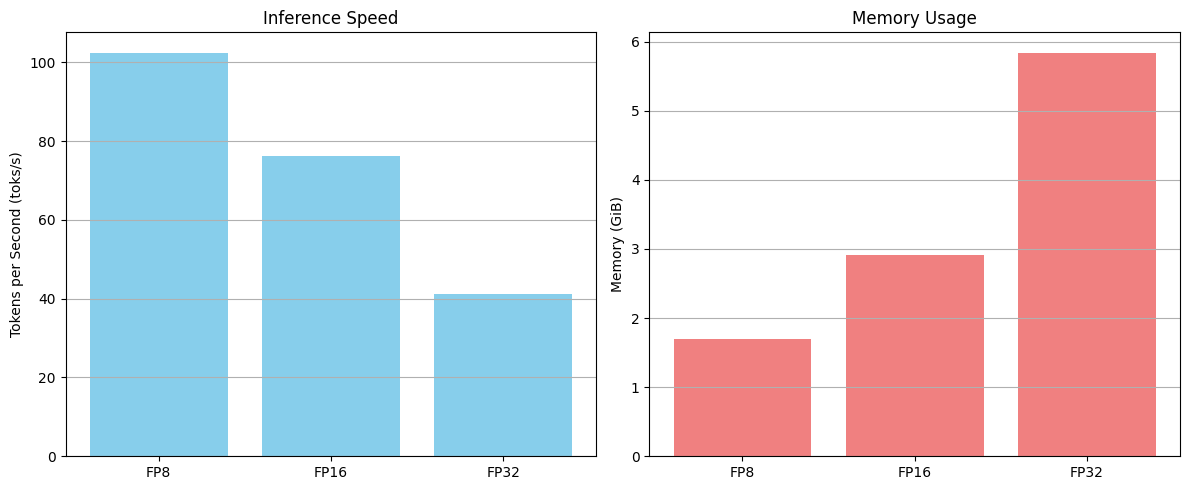
\includegraphics[width=\linewidth]{figures/c4/inference_benchmark.png}
    \caption{Inference speed (higher is better) and memory usage (lower is better) for FP32, FP16, and FP8.}
    \label{fig:inference_benchmark}
\end{figure}
